\documentclass{beamer}

\usefonttheme{professionalfonts} % using non standard fonts for beamer
\usefonttheme{serif} % default family is serif

%\usepackage{hyperref}

%\usepackage{minted}

\usepackage{animate}

\usepackage{graphicx}

\def\Put(#1,#2)#3{\leavevmode\makebox(0,0){\put(#1,#2){#3}}}

\usepackage{color}

\usepackage{tikz}

\usepackage{amssymb}

\usepackage{enumerate}


\newcommand\blfootnote[1]{%

  \begingroup

  \renewcommand\thefootnote{}\footnote{#1}%

  \addtocounter{footnote}{-1}%

  \endgroup

}

\makeatletter

%%%%%%%%%%%%%%%%%%%%%%%%%%%%%% Textclass specific LaTeX commands.

 % this default might be overridden by plain title style

 \newcommand\makebeamertitle{\frame{\maketitle}}%

 % (ERT) argument for the TOC

 \AtBeginDocument{%

   \let\origtableofcontents=\tableofcontents

   \def\tableofcontents{\@ifnextchar[{\origtableofcontents}{\gobbletableofcontents}}

   \def\gobbletableofcontents#1{\origtableofcontents}

 }

%%%%%%%%%%%%%%%%%%%%%%%%%%%%%% User specified LaTeX commands.

\usetheme{Malmoe}

% or ...

\useoutertheme{infolines}

\addtobeamertemplate{headline}{}{\vskip2pt}



\setbeamercovered{transparent}

% or whatever (possibly just delete it)

\makeatother

\begin{document}
\title[SDCEL report]{A Scalable DCEL implementation}
\author[AC]{Andres Calderon}
\institute[Spring'20]{University of California, Riverside}
\makebeamertitle
\newif\iflattersubsect

\AtBeginSection[] {
    \begin{frame}<beamer>
    \frametitle{Outline} 
    \tableofcontents[currentsection]  
    \end{frame}
    \lattersubsectfalse
}

\AtBeginSubsection[] {
    \begin{frame}<beamer>
    \frametitle{Outline} 
    \tableofcontents[currentsubsection]  
    \end{frame}
}

\begin{frame}{Improvements on CGAL implementation...}
    \begin{itemize}
        \item From \textit{CGAL Arrangements and Their Applications: A Step-by-Step Guide}...
        \begin{itemize}
            \item Inserting segments which are disjoint from all of those present in the existing arrangement is quite straightforward...
            \item However, ``Inserting a curve\footnote{A continuous curve $c$ in $\mathbb{R}^2$ is called x-monotone, if every vertical line intersects it at a single point at most.} that intersects with the curves already in the arrangement is much more complicated and requires the application of nontrivial geometric algorithms. (Section 2.2.2 Modifying the Arrangement, pg 26)''
        \end{itemize}
    \end{itemize}
\end{frame}

\begin{frame}{Improvements on CGAL implementation...}
    \centering
	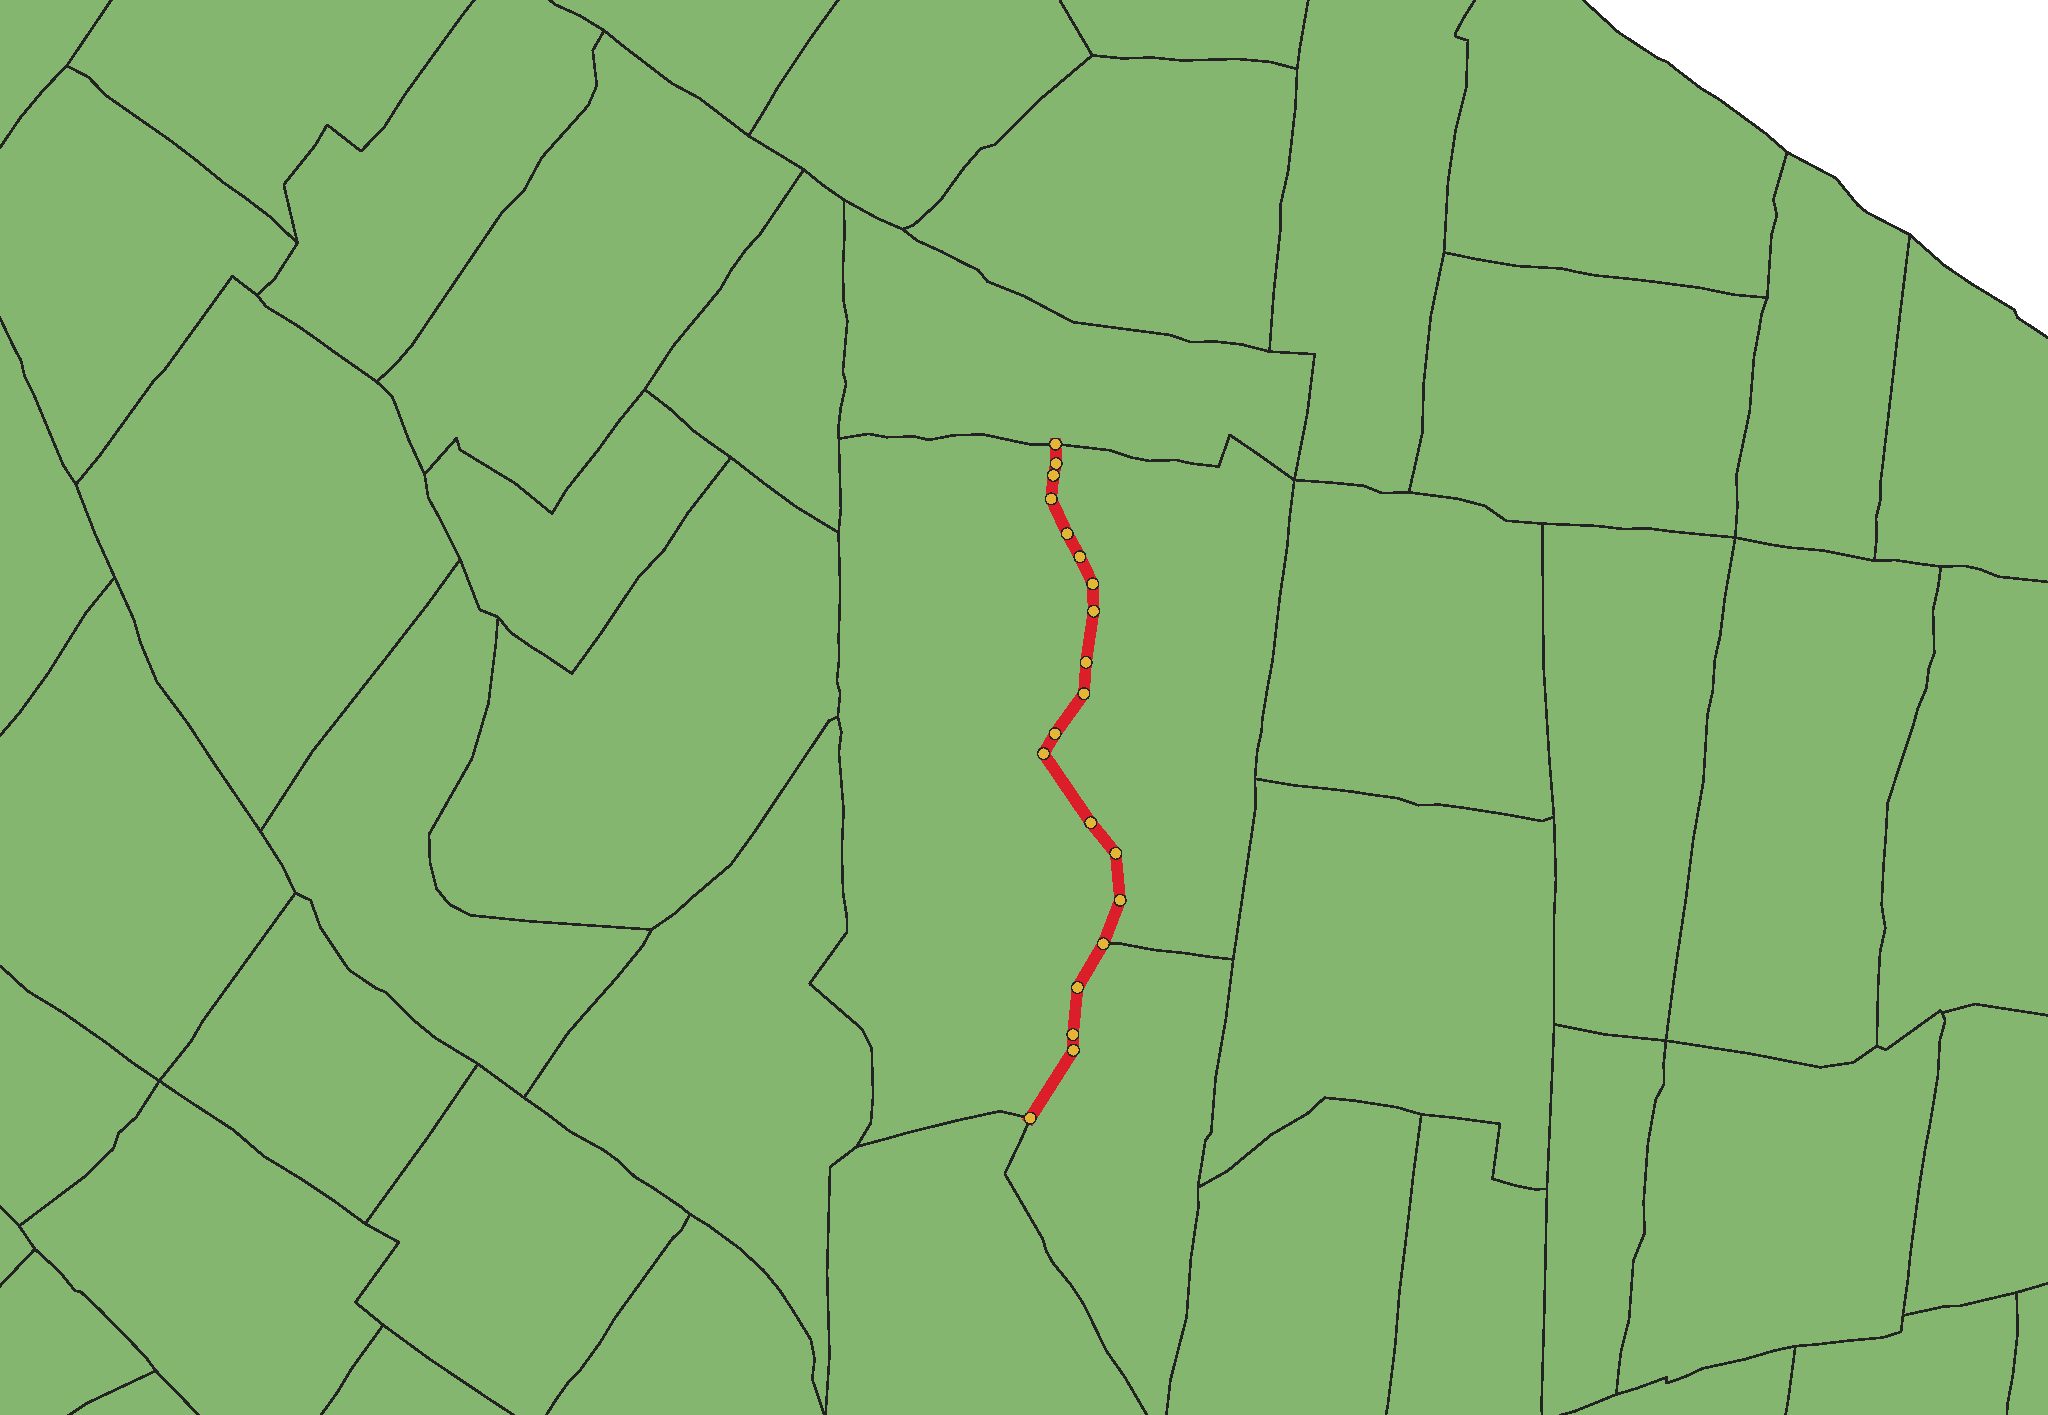
\includegraphics[width=0.8\textwidth]{figures/seg}
\end{frame}

\begin{frame}{Improvements on CGAL implementation...}
    \begin{itemize}
        \item From \textit{CGAL Arrangements and Their Applications: A Step-by-Step Guide}...
        \begin{itemize}
            \item CGAL provides two strategies for insertion of intersecting edges: Incremental (I am using this one) and Aggregate.
            \item But, ``(...) in practice it is recommended that \textbf{the aggregate construction process be used} even for dense arrangements.(Section 3.4.2 Aggregate Insertion Functions, pg 55)''
            \item Aggregate insertion functions do not issue any point-location queries.  The book states: ``there is a trade-off between construction time and query time in each of the point-location strategies, which affects the running times of the incremental insertion process.''
        \end{itemize}
    \end{itemize}
\end{frame}

\begin{frame}{Improvements on CGAL implementation...}
    \begin{itemize}
        \item Indeed, from [1] ... \blfootnote{\tiny [1] \url{https://tinyurl.com/y8m5dqwj}}
        \begin{itemize}
            \item Incremental insertion is based on the zone framework.  It can take $\mathcal{O}(n^2)$.
            \item Aggregate insertion is based on the plane-sweep framework.  It takes $\mathcal{O}((k + n)(\log{} n))$ where $k$ is the number of intersections between the segments.
        \end{itemize}
    \end{itemize}
\end{frame}

\begin{frame}{Working on random edge generator...}
    \centering
	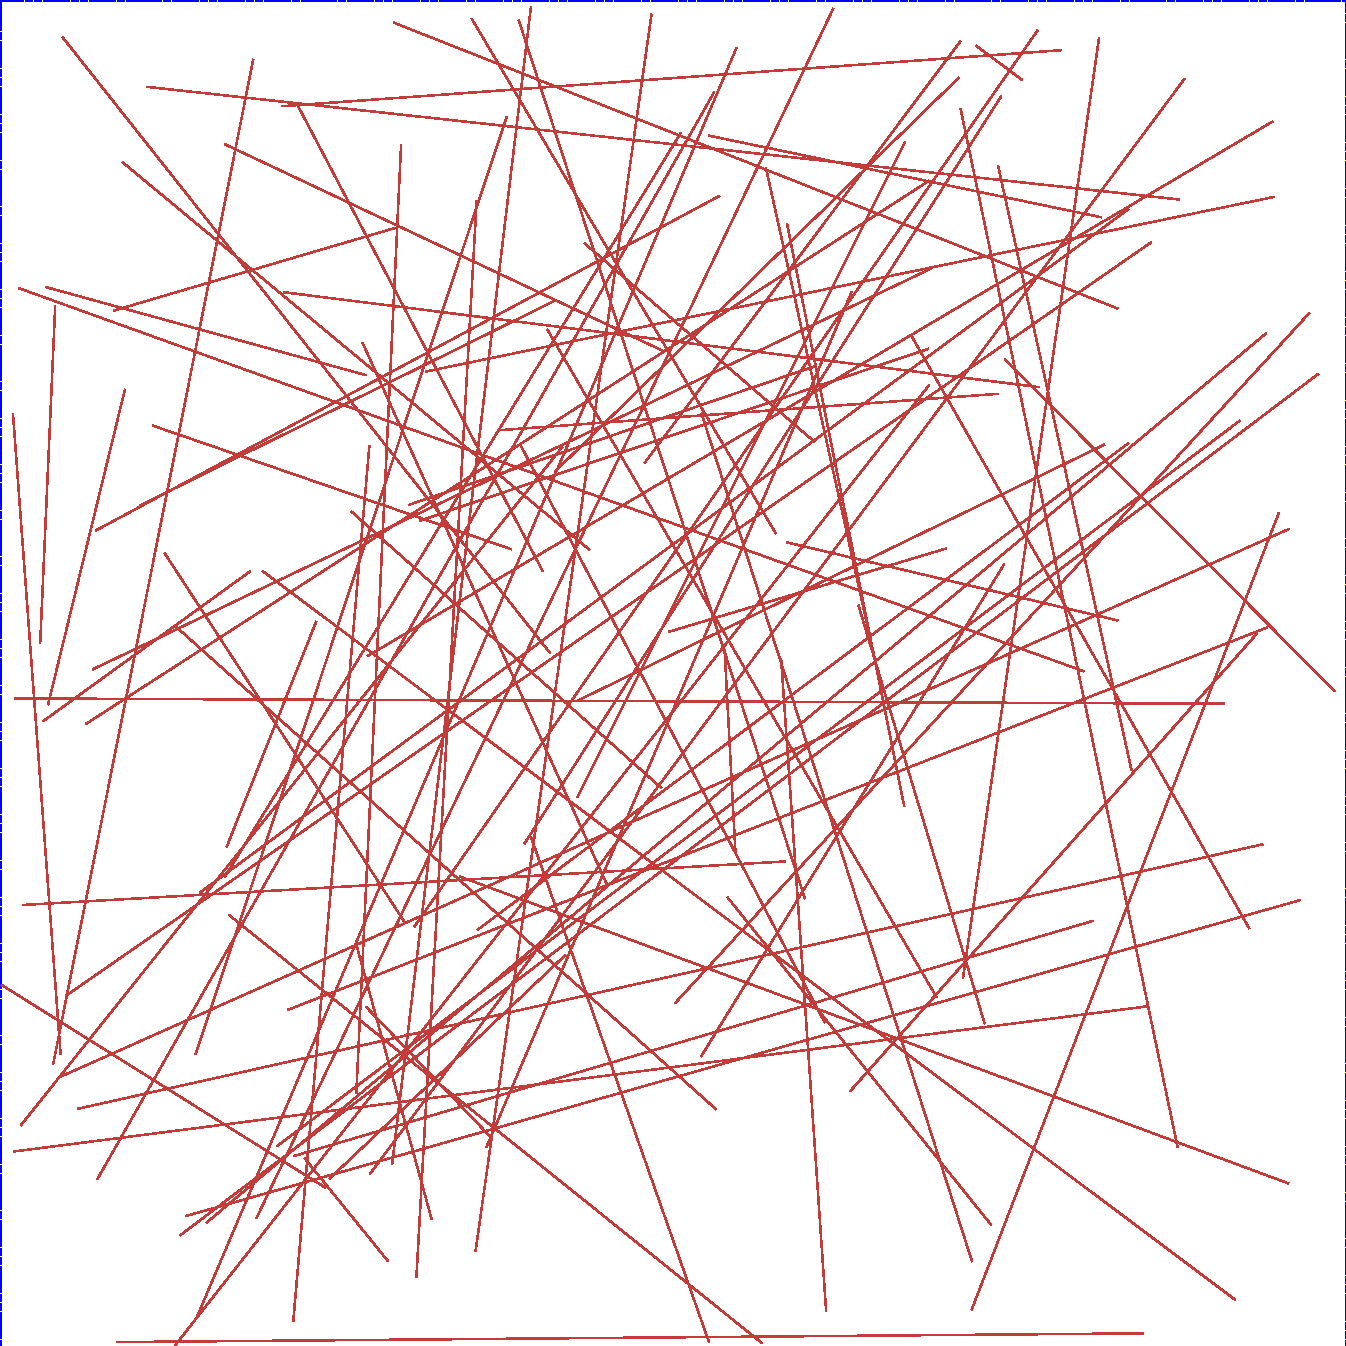
\includegraphics[width=0.6\textwidth]{figures/reg}
\end{frame}

\begin{frame}{What's next...}
    \begin{itemize}
        \item Currently working on the aggregate strategy to read layer of polygons...
        \item Benchmark the new implementation with datasets from the random edge generator...
    \end{itemize}
\end{frame}

\end{document}
